\chapter{矩阵微分}

\section{标量对标量微分$\rightarrow$标量}
\begin{empheq}{align}
\frac{\partial |A(t)|}{\partial t}&=|A|\trace\left(A^{-1}\frac{\partial A}{\partial t}\right)\label{derivative-det}
\end{empheq}
\section{标量对向量微分$\rightarrow$向量}
\begin{empheq}{align*}
\frac{\partial \bm{a}^T\bx}{\partial \bx}&=\frac{\partial \bm{x}^T\bm{a}}{\partial \bx}=\bm{a}\\
\frac{\partial\bx^T A\bx}{\partial \bx}&=(A+A^T)\bx\\
\frac{\partial \ln|A|}{\partial \bx} &=\text{trace}\Big(A^{-1}\frac{\partial A}{\partial \bx}\Big)\\
\frac{\partial G(\bm{w}^T\bx)}{\partial \bm{w}}&=\bx g(\bm{w}^T\bx)\\
\pdv{(\by-\bx)^T\Sigma(\by-\bx)}{\bx}&=-2\Sigma^T(\by-\bx)\\
\pdv{(\by-A\bx)^T\Sigma(\by-A\bx)}{\bx}&=-2A^T\Sigma^T(\by-A\bx)
\end{empheq}

\section{标量对矩阵微分$\rightarrow$矩阵}
$\trace$算子很常见,注意它本身是标量,所以内部可以转置.

\begin{empheq}{align*}
\frac{\partial \text{ trace}(XA)}{\partial X}&=A^T\\
\frac{\partial \text{ trace}(X^TA)}{\partial X}&=\frac{\partial \text{ trace}(AX^T)}{\partial X}=A\\
\frac{\partial \trace(X^TX)}{\partial X}&=\frac{\partial \trace(XX^T)}{\partial X}=2X\\
\frac{\partial \text{ trace}(XBX^T)}{\partial X}&=\frac{\partial \text{ trace}(BX^TX)}{\partial X}=\frac{\partial \text{ trace}(X^TXB)}{\partial X}=X(B+B^T)\\
\frac{\partial \trace AX^TB}{\partial X}&=BA\\
\frac{\partial \ln |A|}{\partial A}&=A^{-T}\\
\frac{\partial |A|}{\partial A}&=|A|A^{-T}\\
\frac{\partial g(U)}{\partial X}&=\left[\frac{\partial g(U)}{\partial x_{ij}}\right]=\left[\sum_{k=1}^{M}\sum_{l=1}^{N}\frac{g(U)}{\partial u_{kl}}\frac{\partial u_{kl}}{\partial x_{ij}}\right]\\
\frac{\partial g(U)}{\partial x_{ij}}&=\trace \left[\left(\frac{\partial g(U)}{\partial U}\right)^T\frac{\partial U}{\partial x_{ij}}\right]
\end{empheq}

以下利用全微分可以容易计算出来。

\begin{empheq}{align}
\pdv{(A\bx)^T(A\bx)}{A}&=\pdv{\trace((A\bx)(A\bx)^T)}{A}=2A\bx\bx^T\\
\pdv{(\by-A\bx)^T(\by-A\bx)}{A}&=\pdv{\trace((\by-A\bx)(\by-A\bx)^T)}{A}=-2\b(y-A\bx)\bx^T\label{vector-regression-target}
\end{empheq}
\begin{empheq}{align}
\pdv{\bm{e}^T\Sigma^{-1}\bm{e}}{\Sigma}&=-\Sigma^{-1}\bm{e}\bm{e}^T\Sigma^{-1}=-(\Sigma^{-1}\bm{e})(\Sigma^{-1}\bm{e})^T
\end{empheq}

\section{向量对向量微分$\rightarrow$矩阵}
\begin{empheq}{align*}
\frac{\partial A\bx}{\partial \bx^T}&=A^T
\end{empheq}

注意向量对向量微分有点类似于J矩阵,$A\bx$和$\bm{x}$都是列向量,但我们把$\bm{x}$转置为行向量,与$A\bx$的每一行匹配起来,形成矩阵.

\section{矩阵对标量微分$\rightarrow$矩阵}
\begin{empheq}{align*}
\frac{\partial AB}{\partial x}&=\frac{\partial A}{\partial x}B+A\frac{\partial B}{\partial x}\\
\frac{\partial A^{-1}}{\partial x}&=-A^{-1}\frac{\partial A}{\partial x}A^{-1}
\end{empheq}
要证明这个公式,首先注意$A^{-1}A=I,\frac{\partial I}{\partial x}=\mathbf{0}$,很容易得到.

\begin{empheq}{align*}
\frac{\partial e^{tA}}{\partial t}&=e^{tA}A
\end{empheq}
注意$e^{tA}$是矩阵。

\section{全微分}
直接求导有一定局限性,比如对于向量函数$\by=A\bx$,$\by$不能直接对$\bx$求导,因为向量对矩阵求导,没有直接定义。但通过全微分就比较好写了:
$$\dif \by=A\dif \bx+(\dif A)\bx$$

\subsection{基本规则}
\subsubsection{Element-wise}
\begin{empheq}{align*}
\dif f(\bx)&=f'(\bx)\odot \dif \bx\\
\dif f(X)&=f'(X)\odot \dif X\\
\dif( \bx\odot\bx)&=2\bx\odot\dif\bx
\end{empheq}

$f$和$f'$都是Element-wise的标量函数,那么$f(\bx)$是一个向量。

\subsubsection{标量全微分与偏导数转换}
\paragraph*{核心原理}
\begin{equation}\label{scalar-diff-core}
\odv{L}{A}=B\iff \dif L=\sum_{i,j}((\dif A)\odot B)=\trace((\dif A)B^T)=\trace(B^T\dif A)
\end{equation}
$L$是标量,$A$是矩阵。据此可以推断
$$\dif L=\bx^T(\dif A)\by\iff \odv{L}{A}=\bx\by^T$$
这是因为$\bx^T(\dif A)\by=\trace(\by\bx^T\dif A)$。

又比如
\begin{empheq}{align*}
\dif L=&\bx^T(\by\odot((\dif A)\bz))\\
=&\bx^T\diag(\by)(\dif A)\bz\\
=&\trace((\dif A)\bz\bx^T\diag(\by))\\
\iff&\odv{L}{A}=\diag(\by)\bx\bz^T
\end{empheq}
\paragraph*{例子}
\begin{empheq}{align*}
L&=\bx^TW^TW\bx\\
\implies \dif L&=\bx^T((\dif W^T)W+W^T\dif W)\bx\\
&=\trace(\bx^T(\dif W^T)W\bx+\bx^TW^T(\dif W)\bx)\\
&=2\trace(\bx^TW^T(\dif W)\bx)\\
&=2\trace(\bx\bx^TW^T\dif W)\\
\implies \odv{L}{W}&=2W\bx\bx^T
\end{empheq}
\begin{empheq}{align*}
L&=\trace(ABA^T)\\
&=\trace((\dif A)BA^T+A(\dif B)A^T+AB(\dif A)^T)\\
&=\trace((\dif A)(BA^T+B^TA^T))+\trace(A(\dif B)A^T)\\
\implies &\odv{L}{A}=A(B+B^T)\\
&\odv{L}{B}=AA^T
\end{empheq}

\subsubsection{向量全微分与偏导数转换}
\paragraph*{核心原理}
\begin{empheq}{align}
\dif \by=A\dif \bx &\iff \pdv{\by}{\bx^T}=A \mtag{不涉标量}
\end{empheq}
涉及标量的情形比较复杂,因为标量与矩阵其实是两种不同的量,其乘法不能约简。以下给出一些基本的推导:
\begin{empheq}{align}
\by&=f(\bx)\bx,\by\in \mathbb{R}^{d\times 1}, \bx \in \mathbb{R}^{d\times 1}\\
\dif \by&=(\dif f(\bx))\bx+f(\bx)\dif \bx\\
&=(\dif \bx^T f'(\bx))\bx+f(\bx)\dif \bx\\
&=\bx((f'(\bx))^T\dif \bx)+f(\bx)\dif \bx\label{scalar-mat-diff-core-1}\\
\iff \odv{\by}{\bx}&=\bx (f'(\bx))^T+f(\bx)I\label{scalar-mat-diff-core-2}
\end{empheq}
注意从\eqref{scalar-mat-diff-core-1}到\eqref{scalar-mat-diff-core-2}的转换与标量全微分转换的式\eqref{scalar-diff-core}非常相似。

根据上面的结果,立即有以下结论:
\begin{empheq}{align}
\by&=f(\bx)A\bx,\by\in \mathbb{R}^{n\times 1},A\in\mathbb{R}^n, \bx \in \mathbb{R}^{d\times 1}\\
\odv{\by}{\bx^T}&=A\bx (f'(\bx))^T+f(\bx)A
\end{empheq}
\subsubsection{微分基本运算法则}
微分运算的一个基本特征是保持维度不变,就是说对标量微分,必然得到标量。那么原式的形式在求微分后也是保持形式不变的,比如原来是标量乘向量,那么根据乘法的法则,微分后两项都是标量乘以向量。

\begin{empheq}{align}
\dif A^{-1}&=-A^{-1}(\dif A)A^{-1}\\
\dif AB&=(\dif A)B+A\dif B\\
\dif |A|&=\trace(|A|A^{-1}\dif A)\\
\dif \ln |A|&=\trace(A^{-1}\dif A)
\end{empheq}

\subsection{实例}
\begin{example}
以下推导在Kalman滤波中用到,假定$A$是变量,$C$是对称矩阵:
\begin{empheq}{align*}
\dif L&=\dif \trace((I-AB)C(I-AB)^T)\\&=\trace(\dif (I-AB)2C(I-AB)^T)\\
&=\trace(-2(\dif A)BC(I-AB)^T)\\
\implies&\odv{L}{A}=-2(I-AB)CB^T
\end{empheq}
\end{example}

\section{自动微分}
\subsection{原理}
\subsubsection{基本要素}
自动微分的基本原理是把计算过程表示为图:
\begin{center}
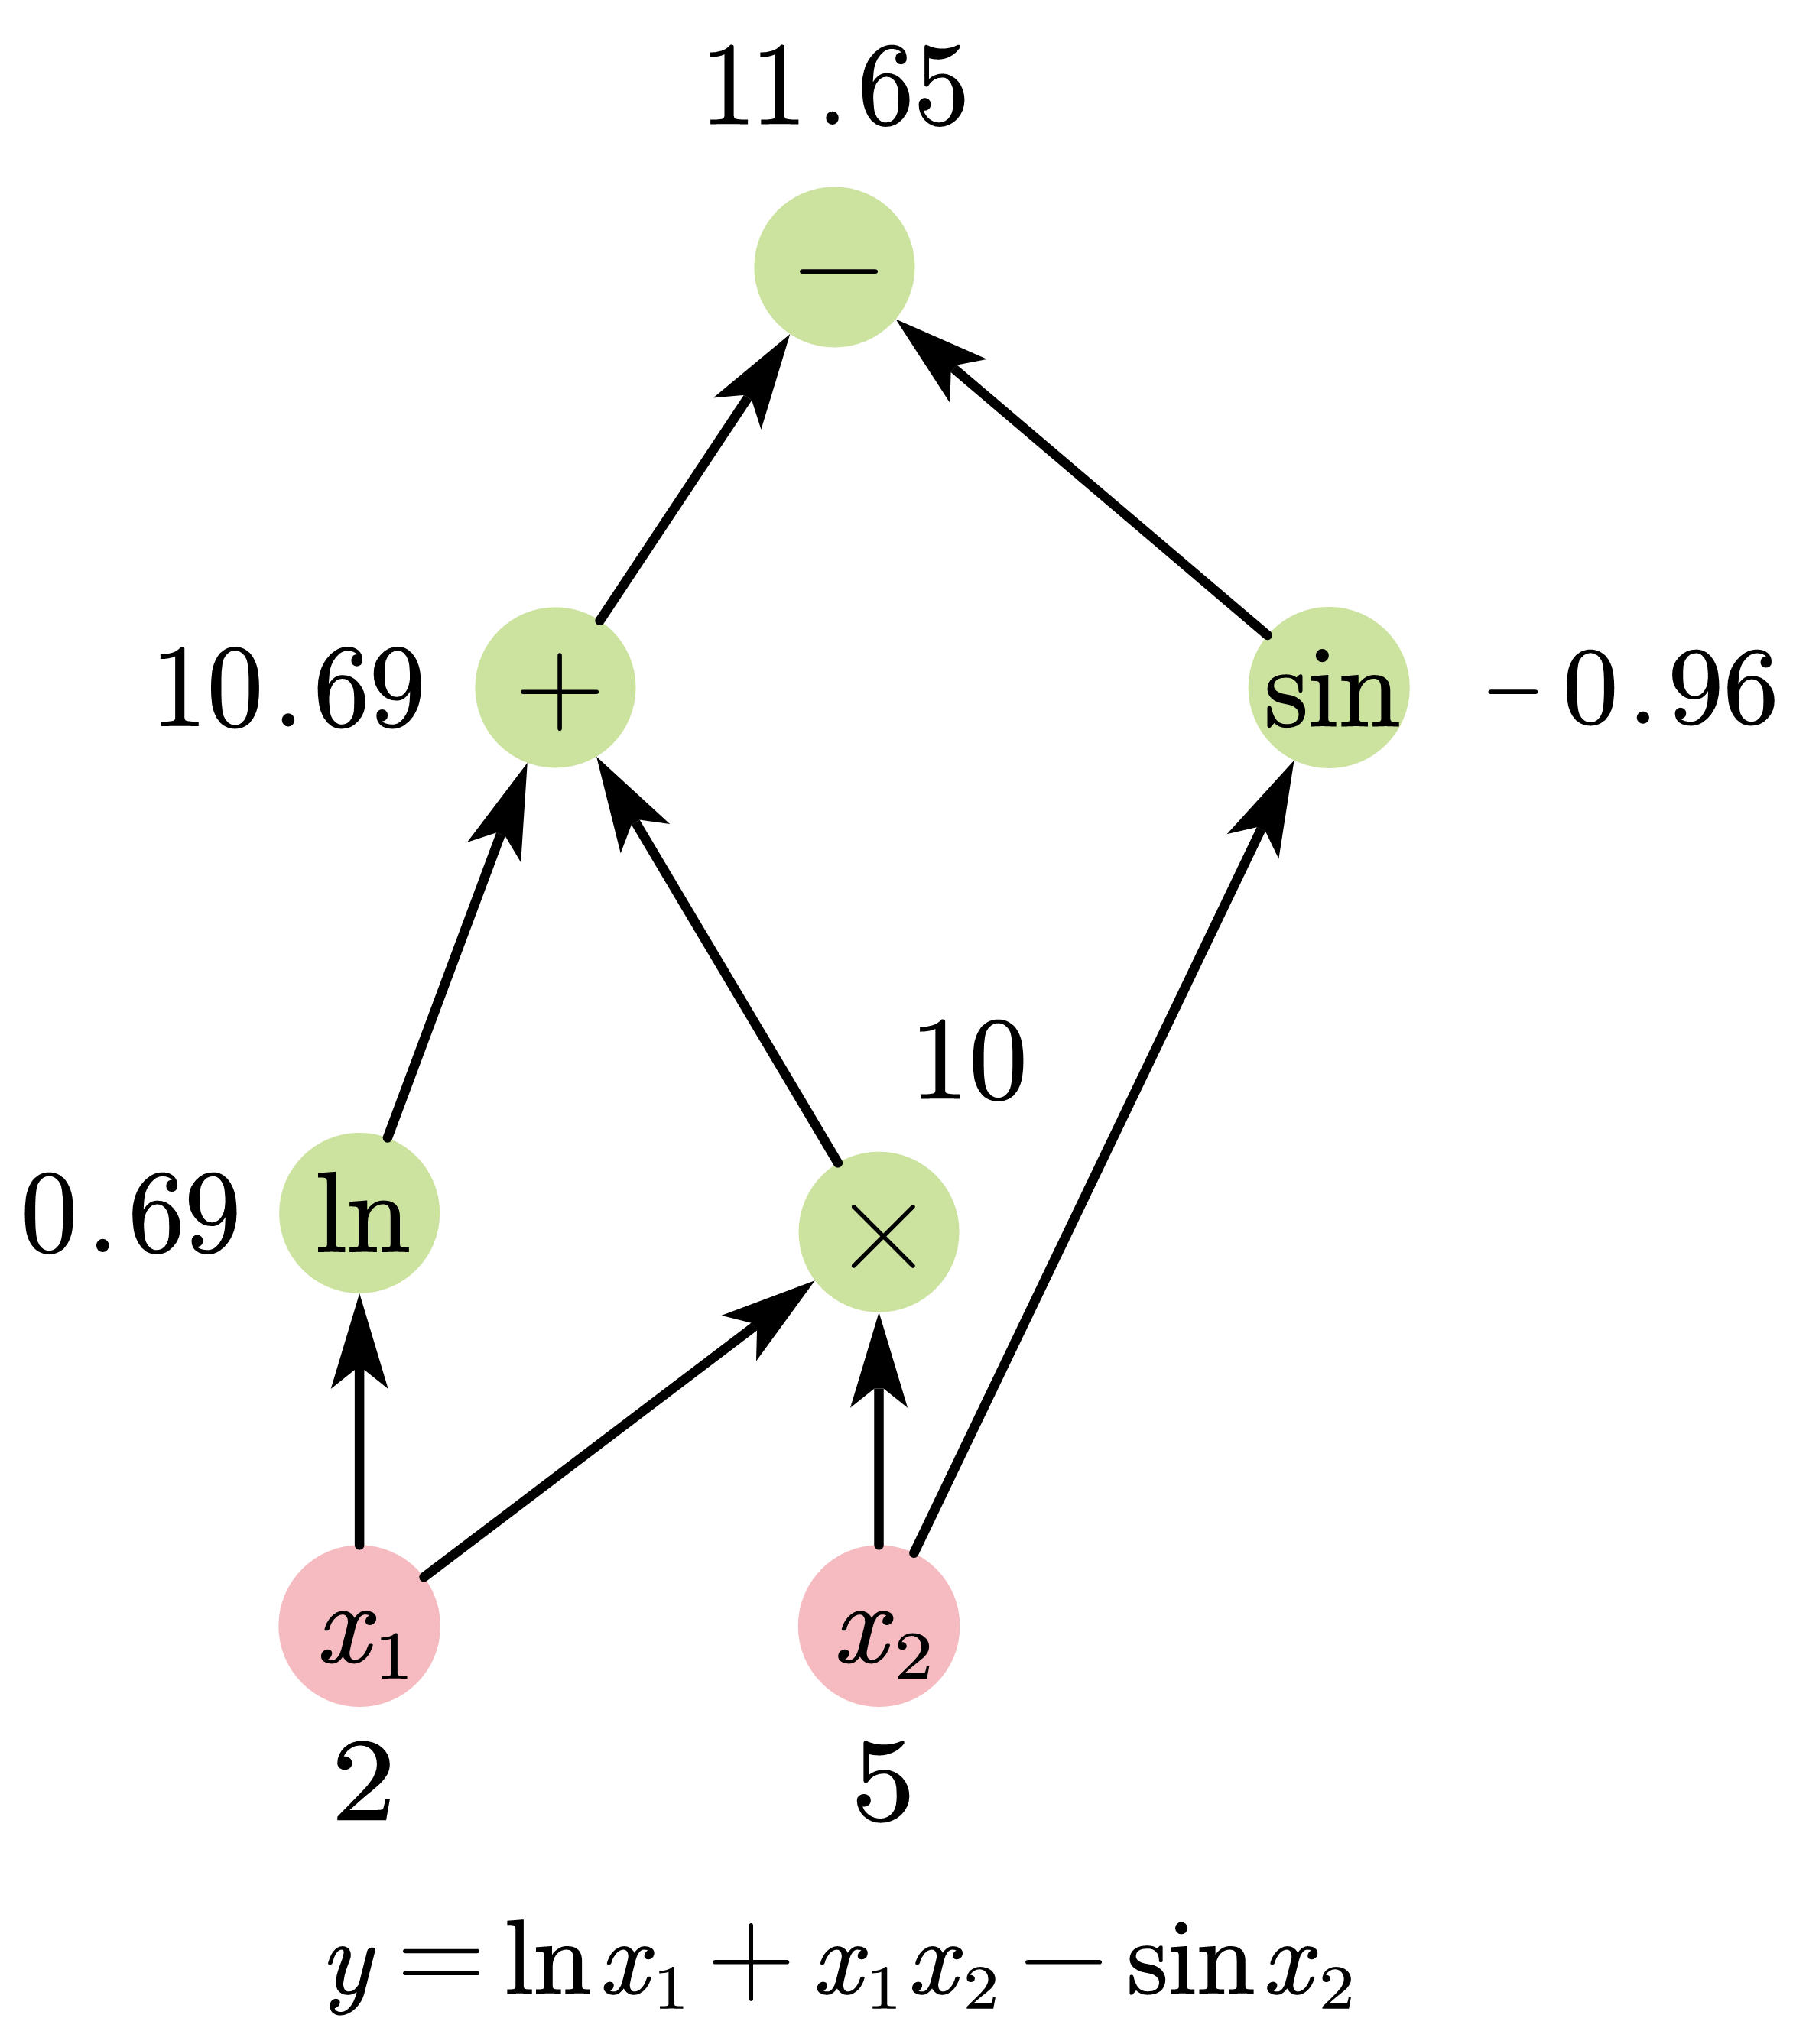
\includegraphics[width=7cm]{figure/ComputingGraph.png}
\end{center}
图有两个基本要素:变量与运算。通过这个图来计算微分,具体计算有两种模式:前向与反向模式。前者是指从变量出发,一次计算中间值与微分;后者是先前向计算函数值,再反向计算微分。反向模式在机器学习中比较常用。

变量可以是张量,包括矩阵、向量在内。图中每个节点只需要存储函数值与微分值。
\subsubsection{反向模式}
计算过程如下:
\begin{center}
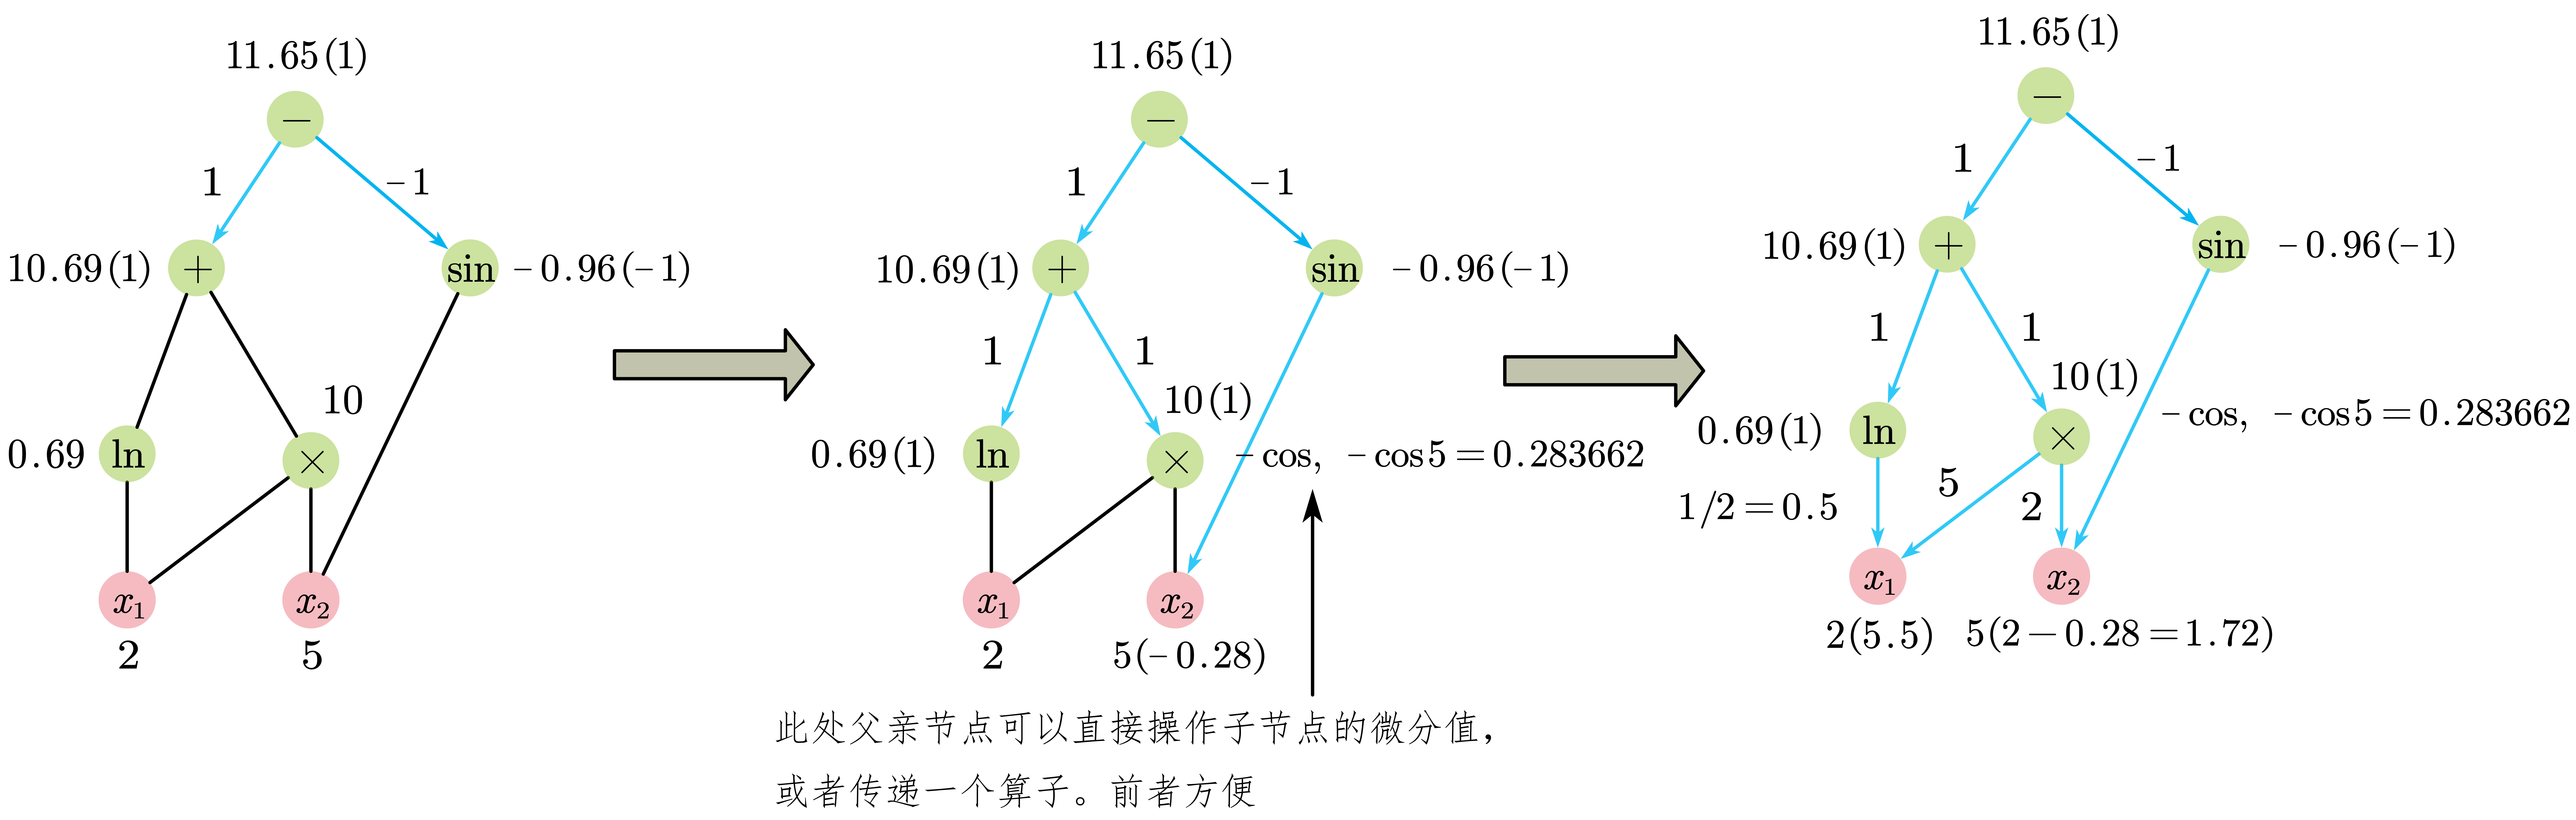
\includegraphics[width=\linewidth]{figure/ReverseMode.png}
\end{center}
节点存储值与微分,父亲节点可以操作子节点的微分值。
\subsubsection{一元运算}

\subsubsection{二元运算}

\subsubsection{矩阵运算}
\paragraph*{转置}转置是很特殊的操作,它本身是一元运算,但它会改变变量的数据结构,所以不能等同于计算图中一个变量输出多条边。
\section{矩阵微分应用实例}
\subsection{神经网络的BP传播}
以下给出一个二次网络的例子:
$$\bm{y}_k=f(\bm{x}_{k-1})=f(g_{k-1}(\by_{k-1}))=f\left(U_{k-1}\by_{k-1}^{\odot 2}+V_{k-1}\by_{k-1}+\bm{b}_{k-1}\right)$$
模型参数是$U_k,V_k,\bm{b}_k$。$\odot$表示Element-wise操作,比如$\bx\odot\by=\diag(\bx)\by$,$\diag(\cdot)$函数假如参数是列向量,则结果是对角矩阵,如果参数是矩阵,结果是对角线构成的列向量。那么$\by_{k-1}^{\odot 2}$表示Element-wise的多项式。注意,这里我们是用的$\by_k$,而不是题目中的$\bx_k$,这是为了方便。$\by_k$为第$k$层在损失函数作用之后的输出,不妨设整个网络输入为第0层,输入为$\bm{y}_0$,最终输出是第$M$层,输出$y_{M}$。于是整个模型表示为

\begin{center}
\begin{tikzcd}[column sep=small]
	\bm{y}_0\arrow[r,"g_0"]& \bm{x}_0 \arrow[r,"f"] & \bm{y}_1\arrow[r,"g_1"]&\bm{x}_1\arrow[r,"f"]&\cdots\arrow[r,"f"]&\bm{y}_{M-1}\arrow[r,"g_{M-1}"]&x_{M-1}\arrow[r,"f"]&y_M\arrow[r,"\mathcal{L}"]&L
\end{tikzcd}
\end{center}
$\mathcal{L}$为损失函数,$L$为最终的损失函数值。可以看出$\bx$的下标数量比$\by$少1。

假如只有一个隐藏层,那么应该是
\begin{center}
	\begin{tikzcd}[column sep=small]
		\bm{y}_0\arrow[r,"g_0"]& \bx_0 \arrow[r,"f"] & \by_1\arrow[r,"g_1"]&x_1\arrow[r,"f"]&y_2\arrow[r,"\mathcal{L}"]&L
	\end{tikzcd}
\end{center}
此时$U_1,V_1$是矩阵,而$U_2,V_2$是行向量,$y_1,x_1$是列向量,$y_2,x_2$是标量。

另外取
\begin{empheq}{align*}
f(x)&=\frac{1}{1+e^{-x}}\\
f'(x)&=f(x)(1-f(x))\\
\mathcal{L}(y_M;y)&=-\left(y\ln y_M+(1-y)\ln(1-y_M)\right)\\
\mathcal{L}'(y_M)&=\frac{1-y}{1-y_M}-\frac{y}{y_M}
\end{empheq}

由于是二分类问题,所以上面取的是损失函数是Binary Cross-Entropy函数。

我们的目标是计算损失对参数的导数,即$\pdv{L}{U_k},\pdv{L}{V_k},\pdv{L}{\bm{b}_k}$
。然后利用梯度下降法来更新:
\begin{empheq}{align}
U_k^{(t+1)}&=U_k^{(t)}-\eta\E\left(\pdv{L}{U_k^{(t)}}\right)\\
V_k^{(t+1)}&=V_k^{(t)}-\eta\E\left(\pdv{L}{V_k^{(t)}}\right)\\
\bm{b}_k^{(t+1)}&=\bm{b}_k^{(t)}-\eta\E\left(\pdv{L}{\bm{b}_k^{(t)}}\right)
\end{empheq}
其中$\E(\cdot)$为期望,可以用在样本点处的导数的均值来代替。

利用全微分,有
\begin{empheq}{align}
\dif \bm{x}_k=&(\dif U_{k}) \by_{k}^{\odot 2}+2U_{k}\diag(\by_{k})\dif \by_{k}+(\dif V_{k}) \bm{y}_{k}+V_{k}\dif \by_{k}+\dif \bm{b}_k\nonumber\\
=&(\dif U_{k}) \by_{k}^{\odot 2}+(2U_{k}\diag(\by_{k})+V_{k})\dif \by_{k} +(\dif V_{k}) \bm{y}_{k}+\dif\bm{b}_{k}\\
\dif \bx_0=&(\dif U_0) \by_{0}^{\odot 2}+(\dif V_0) \bm{y}_{0}+\dif \bm{b}_0\label{total_dif_1}\\
\dif \bm{y}_k=&f'(\bx_{k-1})\odot\dif \bx_{k-1}\label{total_dif_2}\\
\dif L=&\mathcal{L}'(y_M)\dif y_M\label{total_dif_3}
\end{empheq}
强调这里的求导是对于单个样本而言的。

从全微分中得到偏微分时,可以忽略掉不相关的项,比如
$$\dif L=\mathcal{L}'(y_{M})f'(x_{M-1})(dU_{M-1})\by_{M-1}^{\odot 2}+C$$
那么
$$\frac{\partial L}{\partial U_M}=\mathcal{L}'(y_M)f'(x_{M-1})(\by_{M-1}^{\odot 2})^T$$
这里使用了两个技巧。第一,如果$\frac{\dif L}{\dif A}=B$,那么$\dif L=\sum_{i,j}(\dif A\odot B)=\trace(B^T\dif A)=\trace((\dif A)B^T)$,反之亦然。第二,$\bx^T\by=\trace(\bx^T\by)=\trace(\bx\by^T)$。

类似地有:
\begin{empheq}{align}
\pdv{L}{V_M}&=\mathcal{L}'(y_M)f'(x_{M-1})(\by_{M-1})^T\\
\pdv{L}{\bm{b}_M}&=\mathcal{L}'(y_M)f'(x_{M-1})
\end{empheq}

现在考虑$\dif\bx$的展开式中的$\dif \by_{k-1}$项,它展开后,可以得到$\dif U_{k-1},\dif V_{k-1},\dif \by_{k-2}$,前两个项可以用于求偏导。此时
$$\dif L=\mathcal{L}'(y_M)f'(x_{M-1})(2U_{M-1}\diag(\by_{M-1})+V_{M-1})\dif \by_{k-1}+C$$
所以要求$V_{k-1}$的偏导数,就要展开$\dif \by_{k-1}$项。不妨假设$\dif \by_{k}$项的系数矩阵是$A_{k}$,那么
\begin{empheq}{align}
A_M&=\mathcal{L}'(y_M)\label{init0}\\
\dif L&=\mathcal{L}'(y_M)\dif y_M\\
&=A_{k}\dif \by_{k}+C\\
&=A_{k}\diag(f'(\bx_{k-1}))\dif \bx_{k-1}+C
\end{empheq}

那么可以得到
\begin{empheq}{align}
\pdv{L}{\bm{b}_{k-1}}&=\diag(f'(\bx_{k-1}))A_{k}^T\label{rec1}\\
\frac{\partial L}{\partial U_{k-1}}&=\diag(f'(\bx_{k-1}))A_{k}^T(\by_{k-1}^{\odot 2})^T=\pdv{L}{\bm{b}_{k-1}}(\by_{k-1}^{\odot 2})^T\label{rec2}\\
\pdv{L}{V_{k-1}}&=\diag(f'(\bx_{k-1}))A_{k}^T(\by_{k-1})^T=\pdv{L}{\bm{b}_{k-1}}(\by_{k-1})^T\label{rec3}\\
A_{k-1}&= A_{k}\diag(f'(\bx_{k-1}))(2U_{k-1}\diag(\by_{k-1})+V_{k-1})\label{rec4}
\end{empheq}

注意$A_0$其实是没用的,可以从\cref{total_dif_1}看出来,$\dif x_0$的展开式中没有$\dif \bm{y}_0$。

至此,已经给出了反向传播的全部递推式。即由\cref{init0,rec1,rec2,rec3,rec4}可以进行反向传播。在实现的时候,可以把$U_k,V_k,\bm{b}_k,A_k,\bx_{k},\by_k$存储在向量中,然后按下标访问。